\documentclass[10pt,danish]{beamer}
\setbeamercovered{transparent}
\usepackage{bm}
\usepackage{amsmath}
\usepackage{graphics}
\usepackage{avant}
\usepackage{amsfonts}
\usepackage{amsmath}
\usepackage{bm}
\usepackage{times}
\usepackage{verbatim}
\usepackage{amssymb}
\usepackage{multicol}

\usetheme{Boadilla}
\title[Incompleteness phenomena in mathematics]{Incompleteness Phenomena in Mathematics:\\ From Kurt G\"odel to Harvey Friedman}
\author{Lasse Grinderslev Andersen}
\date{August 28th, 2016}
\definecolor{PineGreen}{RGB}{0,159,159}

\newcommand\MyLBrace[2]{%
  \left.\rule{0pt}{#1}\right\}\text{#2}}

\begin{document}
\begin{frame}
\titlepage
\begin{center}

\includegraphics[scale=0.3]{logo.png}
\end{center}
\end{frame}

\begin{frame}[c]
\frametitle{Overview of this talk}
 \begin{itemize}
  \item Genesis of modern rigorous mathematics
  \begin{itemize}
   \item Logic \& formal systems
   \item Basic set theory
  \end{itemize}
  \item Mathematical Incompleteness
  \item Reverse Mathematics (\textbf{optional})
  \item Extremely strong case of (concrete) incompleteness
 \end{itemize}
\end{frame}

\begin{frame}
A few basic objects:
\begin{itemize}
\item Natural numbers: $\mathbb{N}=\{0,1,2,3..\}$
\item Integers: $\mathbb{Z}=\{..., -3,-2, -1,0,1,2,3..\}$
\item Rationals: $\mathbb{Q}=\{\frac{n}{m}|n \in \mathbb{Z}, m \in \mathbb{N} \}$
\item Reals: $\mathbb{R}=\mathbb{Q} \cup \{ \text{The Rest} \}$
\end{itemize}
\end{frame}

\begin{frame}
\frametitle{Genesis of modern rigorous mathematics}
\textbf{The entire concept of function was put into question}:
\begin{exampleblock}{}
  {``By about 1800 the mathematicians began to be concerned
               about the looseness in the concepts and proofs of the vast
               branches of analysis. The very concept of a function was not
	       clear; the use of series without regard to convergence and
	       divergence had produced paradoxes and disagreements''}
  \vskip5mm
  \hspace*\fill{\small--- M. Kline}
 \end{exampleblock}
\end{frame}

\begin{frame}[t]
\frametitle{The work of Cantor}
Generalized the notion of infinity in several ways:
\begin{itemize}
 \item[a] \textbf{Transfinite orderings (ordinals)}
\end{itemize}

\begin{align*}
 & 1,2,3,\ldots,n,\ldots,\omega,\omega +1,\omega +2,\omega +3, \ldots, \omega + n,\ldots,2\cdot\omega,3\cdot\omega,\ldots,n\cdot \omega, \\
 & \ldots,\omega^2,\omega^3,\ldots,\omega^n,\ldots,\omega ^3,\ldots,\omega^{\omega},\omega^{\omega^{\omega}},\omega^{\omega^{\omega^{\omega}}},\ldots
\end{align*}

\noindent
\begin{tabular}{c@{}l}
  \begin{tabular}{ll@{}}
    $\omega^{\omega^{\omega^{\omega^{\omega}}}}$ &  

  \end{tabular} 
  & 
  $\begin{array}{l}
    \MyLBrace{4.4ex}{$\omega \ =\varepsilon_0, \varepsilon_0 + 1,\varepsilon_0 + 2,\varepsilon_0 + 3,\ldots,\varepsilon_0 + n,\ldots,\varepsilon_0 ^{\varepsilon_0},\varepsilon_0 ^{\varepsilon_0^{\varepsilon_0}},\ldots$} \\
  \end{array}$
\end{tabular}
\vskip10pt
\visible<2-3>{\textbf{\alert{More} generally, two kinds exist}
\begin{align*}
\text{Successor:  } S(\alpha) = \alpha \cup \{ \alpha \} \text{  and limit:  }\lambda = \bigcup_{\alpha < \lambda} \alpha \Rightarrow On
\end{align*}}
\visible<3>{
\textbf{The hierachy goes on and on and...}
\begin{align*}
\ldots \ldots \ldots, \omega_1, \ldots \text{where } \omega_1 = \bigcup \alpha \ , \ |\alpha| = \aleph_0 \\
\end{align*}}
\end{frame}

\begin{frame}[t]
\frametitle{The work of Cantor}
Generalized the notion of infinity in two  ways:
\begin{itemize}
 \item[b] \textbf{Different degrees of infinity (cardinals)}
\end{itemize}
\begin{columns}
\column{.5\textwidth}
\only<1,2,4>{\visible<2>{
\begin{align*}
    s_1 &= \alert{\bm{0}} \ 0\ 0\ 0\ 0\ 0\ 0\ 0\ldots\\
    s_2 &= 1\ \alert{\bm{1}}\ 1\ 1\ 1\ 1\ 1\ 1 \ldots\\
    s_3 &= 0\ 1\ \alert{\bm{0}}\ 1\ 0\ 1\ 0\ 0 \ldots\\
    s_4 &= 1\ 0\ 1\ \alert{\bm{0}}\ 1\ 0\ 1\ 1 \ldots\\
    s_5 &= 1\ 1\ 0\ 1\ \alert{\bm{0}}\ 1\ 1\ 1 \ldots\\
    s_6 &= 0\ 0\ 1\ 1\ 0\ \alert{\bm{1}}\ 1\ 0 \ldots\\
    s_7 &= 1\ 0\ 0\ 0\ 1\ 0\ \alert{\bm{0}}\ 0 \ldots\\
    s_8 &= 1\ 0\ 0\ 0\ 1\ 0\ 1\ \alert{\bm{1}} \ldots\\
    &\vdots\\ 
    &\line(1,0){90}\\
    s_{\text{troll}} &= \structure{\bm{1}} \ \structure{\bm{0}}\ \structure{\bm{1}}\ \structure{\bm{1}}\ \structure{\bm{1}}\ \structure{\bm{0}}\ \structure{\bm{1}} \ \structure{\bm{0}} \ldots
\end{align*}
}}
% SEE IF YOU CAN FIX:
\only<3>{
\begin{align*}
	 \text{Input}&: \textbf{1}\ \textbf{2}\ \textbf{3}\ \textbf{4}\ \textbf{5}\ \textbf{6}\ \textbf{7}\ \textbf{8} \\	 
    P_1 &: \alert{\bm{0}} \ 0\ 0\ 0\ 0\ 0\ 0\ 0\ldots\\
    P_2 &: 1\ \alert{\bm{1}}\ 1\ 1\ 1\ 1\ 1\ 1 \ldots\\
    P_3 &: 0\ 1\ \alert{\bm{0}}\ 1\ 0\ 1\ 0\ 0 \ldots\\
    P_4 &: 1\ 0\ 1\ \alert{\bm{0}}\ 1\ 0\ 1\ 1 \ldots\\
    P_5 &: 1\ 1\ 0\ 1\ \alert{\bm{0}}\ 1\ 1\ 1 \ldots\\
    P_6 &: 0\ 0\ 1\ 1\ 0\ \alert{\bm{1}}\ 1\ 0 \ldots\\
    P_7 &: 1\ 0\ 0\ 0\ 1\ 0\ \alert{\bm{0}}\ 0 \ldots\\
    P_8 &: 1\ 0\ 0\ 0\ 1\ 0\ 1\ \alert{\bm{1}} \ldots\\
    &\vdots\\ 
    &\line(1,0){90}\\
    P_{\text{troll}} &= \structure{1} \ \structure{\text{U}}\ \structure{\text{1}}\ \structure{\text{1}}\ \structure{\text{1}}\ \structure{\text{U}}\ \structure{\text{1}} \ \structure{\text{U}} \ldots
\end{align*}}



\column{.55\textwidth}
\centering
\structure<1>{
Countably infinite sets
\begin{align*}
 | \mathbb{N} | = |\mathbb{Z}| = | \mathbb{Q} | = \omega = \aleph_0
\end{align*}}
\structure<2-3>{
Cantors Diagonal argument:
\begin{align*}
 |\mathbb{N}&|<|\mathbb{R}|\\
 |\mathbb{R}| &=| \mathcal{P}(\mathbb{N})| = 2^{\aleph_0}\\
 | \mathcal{P}(X)|& = 2^{|X|} > |X|
\end{align*}}
Cantors continuum hypothesis
\structure<4>{
\begin{align*}
 |\mathbb{R}| = \aleph_1 \text{ or } \aleph_{\alpha+1}=2^{\aleph_{\alpha}} 
\end{align*}
}
\end{columns}
\end{frame}

\begin{frame}
\frametitle{Reception of Cantors work}
The reception of Cantors discoveries were mixed...
\begin{exampleblock}{}
  {``I don't know what predominates in Cantor's theory - philosophy or theology, but I am sure that there is no mathematics there.''}
  \vskip5mm
  \hspace*\fill{\small--- Leopold Kronecker}
\end{exampleblock}
Others were more positive:\\
 \begin{exampleblock}{}
  {``No one shall expel us from the paradise that Cantor has created for us.''}
  \vskip5mm
  \hspace*\fill{\small--- David Hilbert}
 \end{exampleblock}
\end{frame}

\begin{frame}
 \frametitle{Hilbert program and the formalization of mathematics}
Hilbert 'wanted to battle Kronecker on is own playing field':
\begin{itemize}
 \item Formalize (infinitary) mathematics, making it a 'game of symbols'
 \item A game of symbols can be described and investigated by mathematics!
 \item Prove consistency of mathematics by finitary methods
\end{itemize}
\end{frame}

\begin{frame}
 \frametitle{A formal system example: 'MU'}
The alphabet of the \texttt{MU}-system is $\{$\texttt{M,U,I}$\}$ with rules of inference and axiom:
\begin{description}
 \alert<7>{\item[Rule I] Any string ending with \texttt{I}, you may add \texttt{U} at the end.}
 \alert<4,5>{\item[Rule II] Given string \texttt{Mx} beginning with \texttt{M}, \texttt{x} can be duplicated: \texttt{Mxx}}
 \alert<6>{\item[Rule III] If \texttt{III} occur in a string, it may be replaced by \texttt{U}}
 %\item[Rule IV] ...
 \alert<3>{\item[Axiom] \texttt{MI}}
\end{description}
\uncover<2-8>{\begin{columns}
	\column{0.5\textwidth} 
	\begin{theorem}
		MUIU (Notation: 'MU'-system $\bm{\vdash}$ MUIU)
	\end{theorem}

	\begin{proof}
 		\texttt{\alert<3>{MI},\alert<4>{MII},\alert<5>{MIIII},\alert<6>{MUI},\alert<7>{MUIU}}
	\end{proof}
	\begin{block}{Metatheorem}
 		\alert<8>{\texttt{MU} is unprovable in MUI arithmetic.}%this is not incompleteness per se, since we do not have any notion of truth, yet
	\end{block}
\end{columns}}
\end{frame}

\begin{frame}
	\frametitle{First Order Logic}
	The basis of most formal system (or language): $\mathcal{L}_{FOL}$\\
	Logical symbols:
	\begin{itemize}
	\item \textbf{Equality} $=$
	\item \textbf{Connectives} '\textit{or}': $\vee$, '\textit{and}': $\wedge$, '\textit{not}': $\neg$, '\textit{if-then}': $\rightarrow$, '\textit{if-and-only-if}': $\leftrightarrow$
	\item \textbf{Quantifiers} 'for-all': $\forall$, 'there exists': $\exists$
	\item \textbf{Variables} $x,y,z,...$
	\end{itemize}
	Non-logical symbols:
	\begin{itemize}
	\item \textbf{Relations} $R_1, R_2, R_3,\ldots$
	\item \textbf{Functions} $f_1,f_2,f_3,\ldots$
	\end{itemize}
	\textbf{Example:}\\
For relation '$<$' (\textit{larger than}) we have
\begin{equation}
\forall x \forall y \forall z \ (x<y \wedge y<z \rightarrow x<z)
\end{equation}
\end{frame}

\begin{frame}
 \frametitle{Peano Arithmetic}
Standard axioms of arithmetic in language $\mathcal{L}_{PA}$ with signature $0,S,+,*,<$
\begin{description}
  \only<1>{\item[P1] For every $n \neq 0$ there exists a unique $k$ s.t. $n = S(k)$.}
  \only<2,3>{\item[P1] $\forall n \exists !k(n\neq 0 \wedge n=S(k)$)}
  \only<1>{\item[P2] $0$ is not the successor of any $n$}
  \only<2,3>{\item[P2] $\neg \forall n(0=S(n))$}
 \only<1>{\item[P3] For all $n$ we have $n + 0 = n$}
 \only<2,3>{\item[P3]$ \forall n (n + 0 = n)$}
 \only<1>{\item[P4] For all $n,k$ we have $n + S(k) = S(n+k)$}
 \only<2,3>{\item[P4] $\forall n,k (n+S(k) = S(n+k))$}
 \only<1>{\item[P5] For all $n$ we have $n * 0 = 0$}
 \only<2,3>{\item[P5] $\forall n (n * 0 = 0 )$}
 \only<1>{\item[P6] For all $n,k$ we have $n * S(k) = n * k + n$}
 \only<2,3>{\item[P6] $\forall n,k (n*S(k)=n*k+n)$}
 \only<1>{\item[P7] For each formula $\phi ( n)$ if $\phi (0)$ and $\phi (n) \rightarrow \phi(n+1)$ then $\forall n \phi(n)$}
 \only<2,3>{\item[P7] $(\phi(0) \wedge (\phi(n) \rightarrow \phi(n+1)) \rightarrow \forall n \phi(n))$}
 \item[P8] Axioms for the relation $<$...
\end{description}
\begin{itemize}
\item<3> The structure $\mathbb{N} = (\mathbb{N},0',S',+',*',<')$ is a model for $PA$: $\mathbb{N} \models PA$.
\item<3> There exists uncountably many \textit{non-standard} models of $PA$
\item<3> There exits models of $PA$ with arbitrary uncountable cardinality
\end{itemize}
\end{frame}

\begin{frame}
 \frametitle{Zermelo-Fraenkel set theory}
Zermelo-Fraenkel set theory with axiom of choice (ZFC) formulated in $\mathcal{L}_{ZFC}$ with signature $\in$:
\begin{description}
 \item[Pairing/Union] If we have $x,y$ we also have $\{x,y\}$ and $x \cup y$.
 \item[Empty set] There exist an empty set $\emptyset$.
 \item[Infinity] There exist a set $x$ s.t. $\emptyset \in x$ and $\forall y \in x (y \cup \{ x \})$.
 \item[Extensionabilty] Two sets with the same elements are equal.
 \item[Foundation] No set is an element of itself and no infinite descending chains $...x_3 \in x_2 \in x_1 \in x_0$ exist.
 \item[Powerset] For all sets $x$ exists a corresponding set $\mathcal{P}(x)$ of subsets of $x$.
 \item[Seperation] For all sets $a$ and formulas $\phi (x)$ there exists a set $y = \{ z \in a | \phi(z) \}$.
 \item[Replacement] If $F$ is a function and $x$ is a set, then $F''(x)$ is a set ($F''(x) = \{ y | \forall z\in x (y=F(z))\}$.
 \item[Choice] For any set of sets $x$ there exists a function that takes an element $a$ of $x$ as input and outputs a $z \in a$
\end{description}
\end{frame}

\begin{frame}
 \frametitle{Standard model of ZFC}
Models of ZFC are structures $V = (V,\in)$.\\
Construction of a universe of sets by transfinite recursion along $On$
\begin{align*}
 V_0 &= \emptyset \\
 V_{\alpha + 1} &= \mathcal{P}(V_{\alpha})\\
 V_{\lambda} &= \bigcup_{\alpha < \lambda} V_{\alpha}
\end{align*}
\uncover<2>{A couple of remarks:
\begin{itemize}
 \item $V_{2\omega} \models Z$, i.e. all axioms except replacement and choice
 \item There exist a countable model of ZFC!
 \item If $\kappa$ is an \textit{inaccessible} cardinal, $V_{\kappa} \models ZFC$.
\end{itemize}}
\end{frame}

\begin{frame}
 \frametitle{Inaccessible cardinals}
\begin{definition}
A cardinal $\kappa$ is inaccessible if
\begin{enumerate}
\item[1] $\kappa > \aleph_0$
\item[2] For any cardinal $\lambda < \kappa$ we have $2 ^{\lambda} < \kappa$
\item[3] For any union $\lambda$ of $<\kappa$ ordinals, each which is $<\kappa$ we have $\lambda < \kappa$ (Assuming choice)
\end{enumerate} 
\end{definition}

i.e. even larger than $\beth _{\omega}$ in the hierachy given by
\begin{align*}
 \beth _0 &= \aleph _0 \\
 \beth _{\alpha +1} &= 2 ^{\beth _{\alpha}}\\
 \beth _{\lambda}  &= \bigcup _{\alpha<\lambda}\beth_{\alpha} \text{ (where } \lambda\text{ a limit ordnial)}
\end{align*}
\uncover<2>{
 \textit{many} inaccessible cardinals have been discovered, one larger than the other.
}
\end{frame}

\begin{frame}
 \frametitle{Discovery of the incompleteness phenomena}
\uncover<1>{\begin{block}{G\"odels first incompleteness theorem (for $PA$)}
  There exist a sentence $\sigma$ where $\mathbb{N} \models \sigma$ but $PA \nvdash \sigma$(if PA is consistent)
\end{block}}
\uncover<2>{\begin{block}{G\"odels first incompleteness theorem (for $ZFC$)}
There exists sentences $\sigma$ where $V \models \sigma$ but $ZFC \nvdash \sigma$ (if ZFC is consistent)
\end{block}}
\uncover<3-4>{\begin{block}{G\"odels first incompleteness theorem}
  For any r.e. theory $T$ strong enough to prove 'basic properties' of natural numbers, there exists sentences $\sigma$ where $M \models \sigma$ but $T \nvdash \sigma$\\ (if $T$ is consistent)
\end{block}}
\visible<4>{Proof outline:
\begin{itemize} 
 \item Reduce the mechanical workings of the formal system into arithmetic on $\mathbb{N}$.
 \item i.e. assign unique numbers to formulas and sequences of formulas etc.
 \item Construct troll sentence $\sigma$ expressing '$\sigma$ cannot be proved in $T$'.
\end{itemize}}
\end{frame}

\begin{frame}
 \frametitle{A couple of incompleteness examples}
\begin{itemize}
 \item<1> The G\"odel sentence $\sigma$ of his first incompleteness theorem
 \item<2> In every (consistent) system $T$ we have $Con(T)$ incomplete in $T$\\ (G\"odels 2. incompleteness theorem, destroyed Hilberts program)
 \item<3> In every (consistent) system $T$ there exists diophantine equations incomplete in $T$%TO BE FIXED!
 \item<4> Gentzen proved that $PRA + \epsilon_0 \vdash Con(PA)$ thus $PRA + \epsilon_0$ independent of $PA$
 \item<5> G\"odel and P. Cohen proved that $GCH$ and axiom of choice is independent of $ZFC$
 \item<6> 'There exists a ordinal $\kappa$ that is inaccesable' is independent of $ZFC$
 \item<7> Paris and Harrington proved that (a strong) finite ramsey theorem is independent of $PA$ $\leftarrow$ (using non-standard models) \textbf{first non-foundational result}
\end{itemize}
\end{frame}

\begin{frame}
 \frametitle{Harvey Friedman: Reverse mathematics}
Friedman was one of the founders of 'Reverse Mathematics' in the 1970s.\\
The basic idea was:
\begin{itemize}
\item Forward Mathematics (= usual math): Theorems are deduced from axioms. 
\item Reverse Mathematics: Deduce the axioms from the theorem. 
\item A formal system proved equivalent to a theorem cannot be proved in a weaker subsystem: Independence!
\item Classically a hierarchy of subsystems of second order arithmetic $Z_2$ have been used
    (second order = two variables: $n \in \mathbb{N}$ and $X \in \mathcal{P}(\mathbb{N})$)
\end{itemize}
\end{frame}


\begin{frame}
 \frametitle{Subsystems of reverse mathematics}
\small
\begin{definition}[Arithmetical Hierarchy]
\begin{itemize}
\item[\textbf{1}] $\phi$/$\psi$ is a $\Sigma_{0}^{0}$/$\Pi_{0}^{0}$-formula iff every quantifier is bounded
\item[\textbf{2}] For $k \in \omega$, $\phi$ is a $\Sigma_{k}^{0}$-formula (resp. $\Pi_{k}^{0}$-formula)
if it is of the form 
\begin{displaymath}
\exists n_{1} \forall n_{2} \exists n_{3} \cdots
n_{k}\  \psi\ \ (\textrm{respectively}\ \ \forall n_{1} \exists n_{2} \forall n_{3} \cdots
n_{k}\ 
\phi)
\end{displaymath} where $\phi$/$\psi$ is as above.\\
If $\eta,\sigma$ is $\Sigma_{k}^{0}$, $\Pi_{k}^{0}$ and\\
\begin{displaymath}
\eta \leftrightarrow \sigma
\end{displaymath}
they are $\Delta ^0_k$ formulas.
\end{itemize}
Thus formula-complexity increases with $k$ and this is the arithmetical hierarchy.
\end{definition}
\end{frame}

\begin{frame}
 \frametitle{Subsystems of reverse mathematics}
All subsystems are embedded in $Z_2$:
\begin{definition}
\small
\begin{enumerate}
\item[(i)]  The axioms from PA excluding induction
\item[(ii)] The induction axiom:
\begin{displaymath}
\forall X\ (0 \in X \land \forall x\ (n \in X \rightarrow n+1 \in X)) \rightarrow \forall n\ (n \in X) 
\end{displaymath}
\item[(iii)] The comprehension axiom:
\begin{displaymath}
\exists X \forall n\ (n \in X \leftrightarrow \varphi(n))
\end{displaymath}
where $\varphi(n)$ is a $Z_2$-formula in which $X$ does not occur free.
\end{enumerate}
\end{definition}
\textbf{!!}: Problematic standard semantics: $X \in \mathcal{P}(\mathbb{N})$\\
This strong statement can be gradually weakened giving the base systems
\end{frame}


\begin{frame}
 \frametitle{Subsystems of reverse mathematics: $RCA_0$}
The standard base theory for reverse mathematics
\begin{definition}[$RCA_{0}$]
\small
\begin{enumerate}
\item[(i)] The basic (PA) axioms ((i) from before)
\item[(ii)] $\Sigma_1^0$-induction:
\begin{displaymath}
(\phi(0) \land \forall n\  (\phi(n) \rightarrow \phi(n+1))) \rightarrow
\forall n\  \phi(n)
\end{displaymath}
where $\phi(n)$ is $\Sigma_1^0$. 
\item[(ii)] The scheme of $\Delta_{1}^{0}$-comprehension, that is:
\begin{displaymath}
\forall n\ (\phi(n) \leftrightarrow \psi(n)) \rightarrow \exists X
\forall n\  (n \in X \leftrightarrow \phi(n))
\end{displaymath}
where $\phi(n)$ is a $\Sigma_{1}^{0}$-formula, $\psi(n)$ is a
$\Pi_{1}^{0}$-formula
$\psi(n)$.
\end{enumerate}
\end{definition}
\uncover<2>{$RCA_0$ proves in itself various results, e.g.
\begin{itemize}
 \item Picard-Lindel\"of theorem
 \item The intermediate value theorem on continuous real functions
 \item The existence of an algebraic closure for a countable field (but not its uniqueness)
 %\item The Banach?Steinhaus theorem for a sequence of continuous linear operators on separable Banach spaces
\end{itemize}}
\end{frame}

\begin{frame}
 \frametitle{Subsystems of reverse mathematics: $WKL_0$}
\begin{definition}[$WKL_0$]
\begin{itemize}
\item[(i)] The axioms of $RCA_0$.
\item[(ii)] Weak K\"onig's Lemma: Every infinite binary subtree has an infinite path.\\
\end{itemize}
\end{definition}
\uncover<2>{Examples of theorems that $WKL_0$ is provably equivalent to (over $RCA_0$)
\begin{itemize}
 \item G\"odel's completeness theorem
 \item Every countable commutative ring has a prime ideal
 \item A continuous real function on the closed unit interval is Riemann integrable
 \item Peano's theorem on the existence of ODEs
\end{itemize}}
\end{frame}


\begin{frame}
 \frametitle{Subsystems of reverse mathematics: $ACA_0$}
\begin{definition}[$ACA_0$]
\begin{enumerate}
\item[(i)] $RCA_0$ + full second order induction
\item[(ii)] The arithmetical comprehension scheme, that is:
\begin{displaymath}
\exists X \forall n\ (n \in X \leftrightarrow \varphi(n))
\end{displaymath}
where $\varphi(n)$ in an arithmetical formula.
\end{enumerate}
\end{definition}
\uncover<2>{Examples of theorems that $ACA_{0}$ is provably equivalent to (over $RCA_0$)
\begin{itemize}
 \item K\"onigs lemma
 \item Bolzano-Weierstrass theorem
 \item Every countable commutative ring has a maximal ideal.
\end{itemize}}
\end{frame}

\begin{frame}
 \frametitle{Subsystems of reverse mathematics: $ATR_0$}
\begin{definition}[$ATR_0$]
\begin{enumerate}
\item[(i)] $ACA_0$
\item[(iii)] Transfinite recursion of $\theta(n,X)$ along any countable well-ordering
\end{enumerate}
where $\theta(n,X)$ is an arithmetical formula with (at least) one free number and set variable $n,X$.
\end{definition}
\uncover<2>{Examples of theorems that $ATR_0$ is provably equivalent to (over $RCA_0$)
\begin{itemize}
 \item Any two countable well orderings are comparable.
 \item Ulm's theorem for countable reduced Abelian groups.
 \item Various classical results from descriptive set theory
\end{itemize}}
\end{frame}


\begin{frame}
 \frametitle{Friedmans extremely strong concrete statements}
\begin{theorem}[Invariant Maximal Clique Theorem]
 Every order invariant graph $G=(V,E)$ on $\mathbb{Q}[0,n]^k$ has an upper $Z^+$ order invariant maximal clique.
\end{theorem}

\only<1>{
\begin{figure}
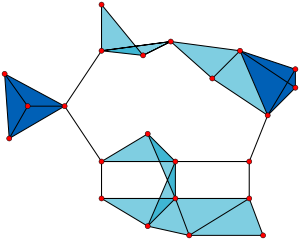
\includegraphics[height=4cm]{clique.png}
\end{figure}}

\only<2>{
\begin{definition}[Order invariant graph]
 $G$ as above is an order invariant graph iff for all order equivalent $x,y \in \mathbb{Q}[0,n]^{2k}$ we have $x \in E \rightarrow y \in E \ (\subseteq \mathbb{Q}[0,n]^{2k})$
\end{definition}
\begin{definition}[Order equivalence]
$x,y \in \mathbb{Q}[0,n]^{2k}$ are order euqivalent if for all $1 \leq i,j \leq  2k \ , \ x_i < x_j \leftrightarrow y_i < y_j$
\end{definition}}

\only<3>{
\begin{definition}[Upper $Z^+$ Order invariant graph]
 $G$ as above is an order invariant graph iff for all upper $Z^+$ order equivalent $x,y \in \mathbb{Q}[0,n]^{2k}$ we have $x \in E \rightarrow y \in E $
\end{definition}
\begin{definition}[Upper $Z^+$ Order equivalence]
$x,y \in \mathbb{Q}[0,n]^{2k}$ are upper $Z^+$ order euqivalent iff they are order equivalent and for all $i$, if $x_i \neq y_i$ then $x_j \geq x_i$, $x_j\geq y_i$, $y_j \geq x_i$ and $y_j \geq y_i$ lies in $Z^+$
\end{definition}}

\only<4>{
\begin{theorem}
 Con(SRP) + ACA' $\vdash$ IMCT and IMCT + ACA' $\vdash$ Con(SRP)
\end{theorem}
here $SRP = ZFC + $ 'there exists extremely large cardinals' and $ACA_0 < ACA' < ATR_0$.}
\end{frame}

\begin{frame}
 \frametitle{Thank you for your attention}
Thanks and dedication to Mette E. Larsen for slides, suggestions and neverending formalist trolling! :-)
\end{frame}

\end{document}
